\section{Modeling problems}

\subsection{Problem 1}
\begin{minipage}{0.45\textwidth}
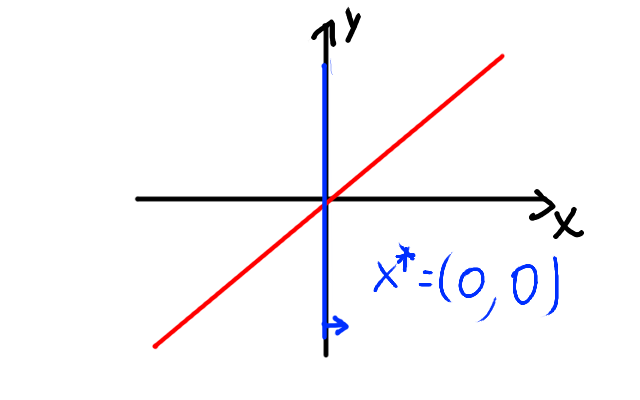
\includegraphics[width=\textwidth]{fig/model/1a.png}
1. a)
\end{minipage}
\hfill
\begin{minipage}{0.45\textwidth}
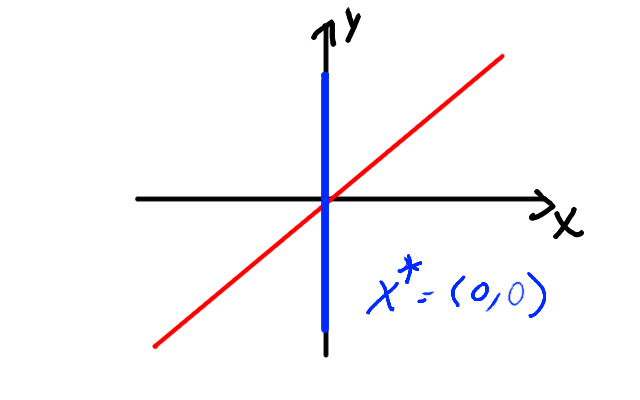
\includegraphics[width=\textwidth]{fig/model/1b.png}
1. b)
\end{minipage}

\begin{minipage}{0.45\textwidth}
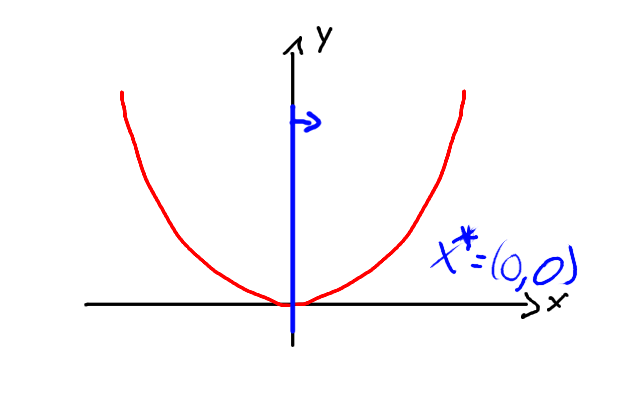
\includegraphics[width=\textwidth]{fig/model/1c.png}
1. c)
\end{minipage}
\hfill
\begin{minipage}{0.45\textwidth}
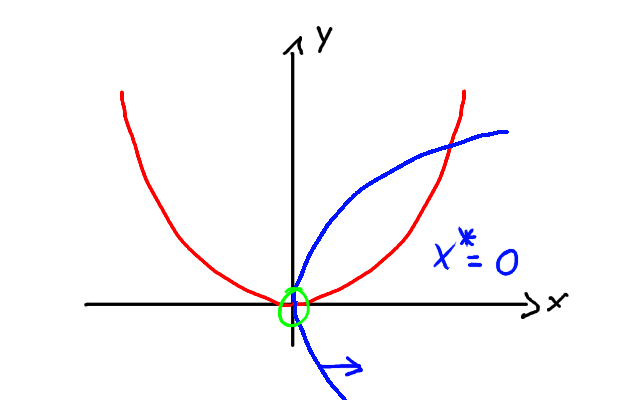
\includegraphics[width=\textwidth]{fig/model/1d.png}
1. d)
\end{minipage}

\begin{minipage}{0.45\textwidth}
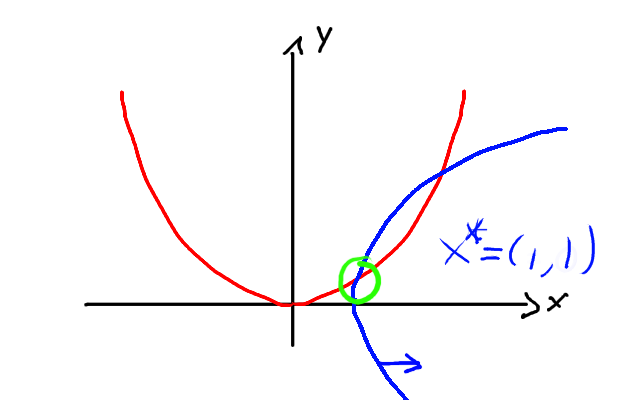
\includegraphics[width=\textwidth]{fig/model/1e.png}
1. e)
\end{minipage}

\pagebreak

\subsection{Problem 2}
\begin{figure}[h]
	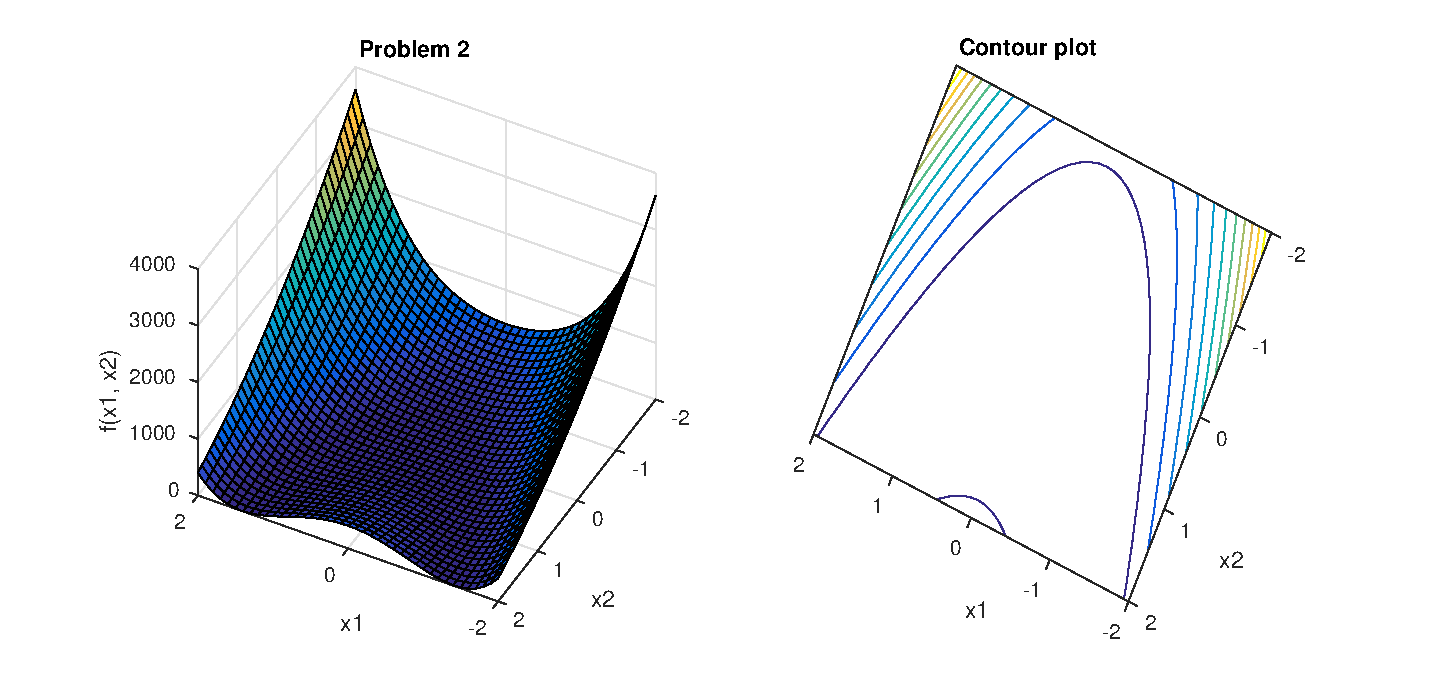
\includegraphics[width=\textwidth]{fig/model/problem2}
\end{figure}

\textbf{2.a)} We see that the two terms containing variables are square therefore the minimum is probably $0$. We can get this result with $x^* = (1,1)$ it is unique because of it is the only root of $100(x_2 - x_1^2)^2 + (1-x_1)^2$.

\textbf{2.b)} 

\lstset{ 
    language=AMPL, % choose the language of the code
    basicstyle=\fontfamily{ttfamily}\selectfont\footnotesize\color{black},
    keywordstyle=\color{blue}\bfseries, % style for keywords
    numbers=left, % where to put the line-numbers
    backgroundcolor=\color{white},
    showspaces=false, % show spaces adding particular underscores
    showstringspaces=false, % underline spaces within strings
    showtabs=false, % show tabs within strings adding particular underscores
    frame=single, % adds a frame around the code
    tabsize=4,
    rulesepcolor=\color{gray},
    rulecolor=\color{black},
    captionpos=b, % sets the caption-position to bottom
    breaklines=true, % sets automatic line breaking
    breakatwhitespace=false, 
}
\begin{lstlisting}
model;

var x1;
var x2;

minimize function:
	100 * (x2 - x1^2)^2 + (1 - x1)^2
\end{lstlisting}

Output:

\begin{lstlisting}[language=]
ampl: model modeling_pb2.mod;
ampl: solve;
MINOS 5.51: optimal solution found.
17 iterations, objective 9.247040366e-19
Nonlin evals: obj = 47, grad = 46.
ampl: display x1, x2;
x1 = 1
x2 = 1
\end{lstlisting}

Which confirms answer in \textbf{2.a)}.

\textbf{2.c)}  Add an equality constraint which changes the solution.
\begin{lstlisting}
model;

var x1;
var x2;

minimize function:
	100 * (x2 - x1^2)^2 + (1 - x1)^2;
	
subject to changeSolutionEqualityConstraint:
	x1 = 2;
\end{lstlisting}

Output:

\begin{lstlisting}[language=]
ampl: model modeling_pb2.mod;
ampl: solve;
MINOS 5.51: optimal solution found.
2 iterations, objective 1
Nonlin evals: obj = 6, grad = 5.
ampl: display x1, x2;
x1 = 2
x2 = 4
\end{lstlisting}

\textbf{2.d)}  Add an equality constraint which \textbf{does not} change the solution.
\begin{lstlisting}
model;

var x1;
var x2;

minimize function:
	100 * (x2 - x1^2)^2 + (1 - x1)^2;
	
subject to dontChangeSolutionEqualityConstraint:
	x1 = 1;
\end{lstlisting}

Output:

\begin{lstlisting}[language=]
ampl: model modeling_pb2.mod;
ampl: solve;
MINOS 5.51: optimal solution found.
2 iterations, objective 0
Nonlin evals: obj = 6, grad = 5.
ampl: display x1, x2;
x1 = 1
x2 = 1
\end{lstlisting}


\textbf{2.e)}  Add an inequality constraint which changes the solution.
\begin{lstlisting}
model;

var x1;
var x2;

minimize function:
	100 * (x2 - x1^2)^2 + (1 - x1)^2;
	
subject to changeSolutionInequalityConstraint:
	x1 >= 2;
\end{lstlisting}

Output:

\begin{lstlisting}[language=]
ampl: model modeling_pb2.mod;
ampl: solve;
MINOS 5.51: optimal solution found.
2 iterations, objective 1
Nonlin evals: obj = 6, grad = 5.
ampl: display x1, x2;
x1 = 2
x2 = 4
\end{lstlisting}

\textbf{2.f)}  Add an inequality constraint which \textbf{does not} changes the solution.
\begin{lstlisting}
model;

var x1;
var x2;

minimize function:
	100 * (x2 - x1^2)^2 + (1 - x1)^2;
	
subject to dontChangeSolutionInequalityConstraint:
	x1 <= 2;
\end{lstlisting}

Output:

\begin{lstlisting}[language=]
ampl: model modeling_pb2.mod;
ampl: solve;
MINOS 5.51: optimal solution found.
17 iterations, objective 9.247040366e-19
Nonlin evals: obj = 47, grad = 46.
ampl: display x1, x2;
x1 = 1
x2 = 1
\end{lstlisting}

\subsection{Problem 3}

Model:

\begin{lstlisting}
model;

var x1;
var x2;

minimize function:
	(x1 - 2)^2 + (x2 -1)^2;
	
subject to zeroConstraint:
	x1^2 - x2 <= 0;
	
subject to twoConstraint:
	x1 + x2 <= 2;
\end{lstlisting}

Output:

\begin{lstlisting}[language=]
ampl: model modeling_pb3.mod;
ampl: solve;
MINOS 5.51: optimal solution found.
12 iterations, objective 1
Nonlin evals: obj = 33, grad = 32, constrs = 33, Jac = 32.
ampl: display x1, x2;
x1 = 1
x2 = 1
\end{lstlisting}

\subsection{Problem 4}

\textbf{4.a)}

\begin{align*}
P_3(x) &= \frac{f^{(0)}(x_0)}{0!} + \frac{f^{(1)}(x_0)}{1!}(x - x_0) + \frac{f^{(2)}(x_0)}{2!}(x - x_0)^2 + \frac{f^{(3)}(x_0)}{3!}(x - x_0)^3\\
&= \cos(1) + \frac{-\sin(1)}{1} (x-1) + \frac{-\cos(1)}{2} (x - 1)^2 + \frac{\sin(1)}{6}(x-1)^3\\
\text{For x = 1.1 we have}\\
P_3(1.1) &= \cos(1) + (-0.0841) + (-0.0027) + (0.0001)\\
&= 0.4536
\end{align*}

\textbf{4.b)}

\begin{align*}
f(x) &= \cos(x) \\
f'(x) &= \sin(\frac{1}{x}) \frac{1}{x^2}\\
f''(x) &= \Big( \sin(\frac{1}{x}) \Big)' \frac{1}{x^2} + \sin(\frac{1}{x}) \Big( \frac{1}{x^2}\Big)'\\
&= \cos(\frac{1}{x})\frac{-1}{x^2}\frac{1}{x^2} + \sin(\frac{1}{x}) \frac{-2}{x^3}\\
&= -\frac{\cos(\frac{1}{x}) + 2x\sin(\frac{1}{x})}{x^4}
\end{align*}

Thus the 2nd order Taylor expansion with $x_0 = 1$ is
\begin{align*}
P_2(x) = \cos(1) + \sin(1)(x-1) + \frac{cos(1) - 2sin(1)}{2}(x - 1)^2
\end{align*}

And for $x = 1.1$ we have
\begin{align*}
P_2(1.1) &= \cos(1) + \sin(1)(1.1-1) + \frac{cos(1) - 2sin(1)}{2}(1.1 - 1)^2\\
&= 0.5403 + 0.0841 - 0.0057\\
&= 0.6187
\end{align*}

\incomplete








